\section{Auswertung}
\label{sec:Auswertung}

\subsection{Bestimmung von Widerständen mittels Wheatstone-Brücke}
Die verschiedenen Werte für die Widerstände $R_3$, $R_4$ und $R_2$, die zur Berechnung des Widerstandes $R_X$
nötig sind, befinden sich in Tabelle \ref{taba}. Dabei beziehen sich die ersten drei Zeilen auf den Widerstand
$R_{X1}$ und die letzten drei auf den Widerstand $R_{X2}$. Für jeden Widerstand $R_X$ werden drei verschiedene
Widerstände $R_2$ verwendet.
\begin{table}\caption{Die Länge der Zylinder und die Spannung mit den jeweiligen Zeitenpunkten der Ausschläge.}
\label{taba}
\centering
\sisetup{round-mode = places, round-precision=2, round-integer-to-decimal=true}
\begin{tabular}{S[]S[]S[]S[]S[]} 
\toprule
{$l/ \si{\milli\meter}$} & {$U_1/ \si{\volt}$} & {$t_1/ \si{\micro\second}$} & {$U_2/ \si{\volt}$} & {$t_2/ \si{\micro\second}$}\\
\midrule
120.8 & 1.29 & 0.6 & 0.17 & 88.7\\
102.3 & 1.27 & 0.5 & 0.2 & 76.5\\
80.5 & 1.33 & 0.6 & 0.76 & 59.8\\
40.4 & 1.33 & 0.5 & 1.34 & 30.2\\
31.1 & 1.29 & 0.5 & 1.37 & 23.8\\
\bottomrule
\end{tabular}\end{table}
\noindent Die gesuchten Widerstände lassen sich daraus mit Gleichung \eqref{eqn:a_r} berechnen.
Für den ersten Widerstand ergibt sich
\begin{equation*}
    R_{X1} = \SI{319.8 \pm 1.2}{\ohm}.
\end{equation*}
Der zweite Widerstand berechnet sich zu
\begin{equation*}
    R_{X2} = \SI{899 \pm 9}{\ohm}.
\end{equation*}

\subsection{Bestimmung von Kapazitäten mittels Kapazitätsmessbrücke}
Die Werte zur Berechnung der Kapazität und des Verlustwiderstandes sind in Tabelle \ref{tabb} aufgelistet.
Für alle drei Kapazitäten $C_2$ liegen jeweils drei Messreihen vor.
\begin{table}\caption{Die angelegte Spannung des elektrischen Feldes innerhalb des Geiger-Müller-Zählrohrs, die Anzahl der jeweils gemessenen Impulse und der Strom innerhalb des Geiger-Müller-Zählrohrs.}
\label{tabb}
\centering
\sisetup{round-mode = places, round-precision=2, round-integer-to-decimal=true}
\begin{tabular}{c c S[]} 
\toprule
{$U / \si{\volt}$} & {$\frac{N}{\SI{130}{\second}}$} & {$I / \si{\ampere}$}\\
\midrule
320 & 11298 & 0.1\\
400 & 11820 & 0.2\\
480 & 12135 & 0.3\\
540 & 12301 & 0.35\\
560 & 12068 & 0.4\\
600 & 12354 & 0.45\\
640 & 12403 & 0.5\\
660 & 12507 & 0.55\\
680 & 12659 & 0.6\\
\bottomrule
\end{tabular}\end{table}
\noindent Der Verlustwiderstand lässt sich mittels Gleichung \eqref{eqn:b_r} zu
\begin{equation*}
    R_X = \SI{510 \pm 40}{\ohm}
\end{equation*}
berechnen.
Die Kapazität ergibt sich mit Gleichung \eqref{eqn:b_c} zu
\begin{equation*}
    C_X = \SI{293 \pm 26}{\nano\farad}.
\end{equation*}

\subsection{Bestimmung von Induktivitäten mittels Induktivitätsmessbrücke}
Für die Berechnung des Verlustwiderstandes sowie der Induktivität einer Spule werden zwei verschiedene
Induktivitäten $L_2$ verwendet. Die Messdaten befinden sich in Tabelle \ref{tabc}.
\begin{table}\caption{Der Anodenstrom und der Kathodenstrom bei einer Beschleunigungsspannung von $U_\text{B} = \SI{25}{\kilo\volt}$ und einer Kathodenspannung $U_\text{K,1} = \SI{500}{\volt}$ und einer Kathodenspannung $U_\text{K,2} = \SI{300}{\volt}$ bei einem Blendenradius von $r_\text{B} = \SI{5}{\milli\meter}$.}
\label{tabc}
\centering
\sisetup{round-mode = places, round-precision=2, round-integer-to-decimal=true}
\begin{tabular}{S[]S[]S[]} 
\toprule
{$I_\text{K} / \si{\milli\ampere}$} & {$I_\text{K,1} / \si{\nano\ampere}$} & {$I_\text{K,2} / \si{\nano\ampere}$}\\
\midrule
1.0 & 2.6 & 2.4\\
0.95 & 2.5 & 2.4\\
0.9 & 2.4 & 2.2\\
0.85 & 2.3 & 2.1\\
0.8 & 2.2 & 2.0\\
0.75 & 2.1 & 1.9\\
0.7 & 1.9 & 1.8\\
0.65 & 1.8 & 1.6\\
0.6 & 1.6 & 1.5\\
0.55 & 1.5 & 1.4\\
0.5 & 1.4 & 1.3\\
0.45 & 1.2 & 1.2\\
0.4 & 1.1 & 1.0\\
0.35 & 0.9 & 0.9\\
0.3 & 0.8 & 0.8\\
0.25 & 0.6 & 0.6\\
0.2 & 0.5 & 0.5\\
0.15 & 0.4 & 0.4\\
0.1 & 0.1 & 0.2\\
0.05 & 0.1 & 0.1\\
\bottomrule
\end{tabular}\end{table}
\noindent Der Verlustwiderstand wird mit Gleichung \eqref{eqn:c_r} berechnet:
\begin{equation*}
    R_X = \SI{100 \pm 4}{\ohm}.
\end{equation*}
Für die Induktivität ergibt sich mit Gleichung \eqref{eqn:c_l}
\begin{equation*}
    L_X = \SI{26.9 \pm 0.8}{\milli\henry}.
\end{equation*}

\subsection{Bestimmung von Induktivitäten mittels Maxwell-Brücke}
Für die erneute Berechnung der Induktivität und des Verlustwiderstandes mit der Maxwell-Brücke werden der Widerstand
$R_2 = \SI{1.0}{\kilo\ohm}$ und die Kapazität $C_4 = \SI{992}{\nano\farad}$ verwendet.
Die eingestellten Widerstände $R_3$ und $R_4$ befinden sich in Tabelle \ref{tabd}.
\begin{table}\caption{Laufzeiten und Spannungen der reflektierten Impulse bei dem Modell des Auges.}
\label{tabd}
\centering
\sisetup{round-mode = places, round-precision=2, round-integer-to-decimal=true}
\begin{tabular}{S[]S[]} 
\toprule
{$t_1/ \si{\micro\second}$} & {$U_1/ \si{\volt}$}\\
\midrule
1.0 & 1.38\\
11.7 & 1.0\\
16.1 & 1.25\\
22.9 & 0.95\\
72.2 & 0.4\\
\bottomrule
\end{tabular}\end{table}
\noindent Der Verlustwiderstand, welcher mit Gleichung \eqref{eqn:d_r} berechnet wird, ergibt sich zu
\begin{equation*}
    R_X = \SI{98.9 \pm 1.8}{\ohm}.
\end{equation*}
Die mit Gleichung \eqref{eqn:d_l} errechnete Induktivität ist
\begin{equation*}
    L_X = \SI{26.1 \pm 0.5}{\milli\henry}.
\end{equation*}

\subsection{Bestimmung der Frequenzabhängigkeit der Brückenspannung mittels Wien-Robinson-Brücke}
Es werden die folgenden Bauteile verwendet:
$R' = \SI{332}{\ohm}$, $2R' = \SI{664}{\ohm}$, $R = \SI{1}{\kilo\ohm}$
und $C = \SI{420}{\nano\farad}$. Die Speisespannung beträgt $U_S = \SI{2.5}{\volt}$.
Die doppelte Brückenspannung in Abhängigkeit von der Frequenz ist in Tabelle \ref{tabe} dargestellt.
Die Werte $\omega / \omega_0$ und $U_{Br} / U_S$ befinden sich in Tabelle \ref{tab1}, wobei die Spannung $U_S = \SI{2.5}{\volt}$ ist.
$\omega_0$ ist dabei die Frequenz, bei der das Brückenspannungsminimum liegt:
\begin{equation*}
    \omega_{0,exp} = \SI[per-mode=fraction]{2513.27}{\per\second}.
\end{equation*}
 Der mittels Gleichung \eqref{omega0} theoretisch errechnete Wert für $\omega_0$ liegt bei 
 \begin{equation*}
     \omega_{0,theo} = \SI[per-mode=fraction]{2380.95}{\per\second}.
 \end{equation*}
\begin{table}\caption{Die Frequenz gegen den doppelten Wert der Amplitude der Brückenspannung.}
\label{tabe}
\centering
\sisetup{round-mode = places, round-precision=3, round-integer-to-decimal=true}
\begin{tabular}{S[]S[]} 
\toprule
{$f/\si{\Hz}$} & {$2 U_{Br}/\si{\V}$}\\
\midrule
20.0 & 1.68\\
50.0 & 1.62\\
100.0 & 1.32\\
150.0 & 0.952\\
200.0 & 0.664\\
250.0 & 0.404\\
300.0 & 0.248\\
400.0 & 0.0608\\
500.0 & 0.304\\
600.0 & 0.492\\
700.0 & 0.636\\
800.0 & 0.8\\
900.0 & 0.896\\
1000.0 & 0.96\\
1100.0 & 1.01\\
1200.0 & 1.04\\
1300.0 & 1.09\\
1400.0 & 1.13\\
1500.0 & 1.2\\
1600.0 & 1.19\\
1700.0 & 1.19\\
1800.0 & 1.22\\
1900.0 & 1.23\\
2000.0 & 1.28\\
2500.0 & 1.31\\
3000.0 & 1.37\\
4000.0 & 1.42\\
5000.0 & 1.41\\
6000.0 & 1.46\\
7000.0 & 1.41\\
10000.0 & 1.38\\
11000.0 & 1.35\\
12000.0 & 1.37\\
13000.0 & 1.34\\
14000.0 & 1.27\\
15000.0 & 1.31\\
16000.0 & 1.28\\
17000.0 & 1.31\\
18000.0 & 1.35\\
19000.0 & 1.35\\
20000.0 & 1.35\\
21000.0 & 1.35\\
22000.0 & 1.35\\
30000.0 & 1.35\\
\bottomrule
\end{tabular}\end{table}
\begin{table}\caption{Der maximale Drehimpuls $L$, der Gesamtspin $S$ und der Gesamtdrehimpuls $J$ ergeben sich zum Landé-Faktor $g_\text{J}$ für die vier verschiedenen Elemente.}
\label{tab1}
\centering
\sisetup{round-mode = places, round-precision=2, round-integer-to-decimal=true}
\begin{tabular}{S[]S[]S[]S[]} 
\toprule
{$L$} & {$S$} & {$J$} & {$g_\text{J}$}\\
\midrule
5.0 & 1.0 & 4.0 & 0.8\\
0.0 & 3.5 & 3.5 & 2.0\\
6.0 & 1.5 & 4.5 & 0.7272727272727273\\
5.0 & 2.5 & 7.5 & 1.3333333333333333\\
\bottomrule
\end{tabular}\end{table}
\noindent Die Werte aus Tabelle \ref{tab1} sind in Abbildung \ref{fig:plot} gegeneinander aufgetragen.
\begin{figure}
 \centering
 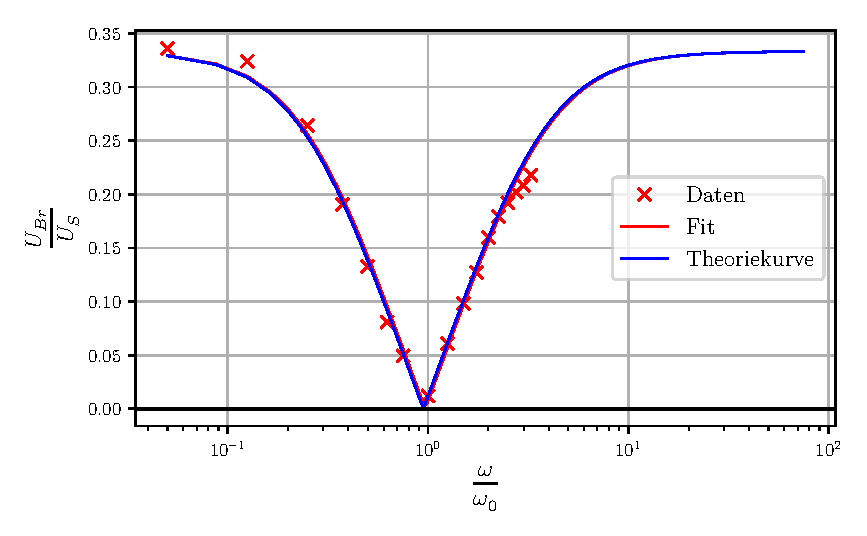
\includegraphics[width= 13cm, height= 9cm]{build/plot1.pdf}
 \caption{$U_{Br}/U_S$ ist gegen $\omega / \omega_0$ aufgetragen. Es sind die Daten, ein Fit und die
 Theoriekurve eingezeichnet.}
 \label{fig:plot}
\end{figure}

\subsection{Bestimmung des Klirrfaktors}
Der minimale Wert der Brückenspannung liegt bei $U_{Br,Min} = \SI{30.4}{\milli\volt}$ bei einer Frequenz von 
$\omega_0 = 2 \pi \cdot 400$. 
\newline
Der Klirrfaktor, der mit Gleichung \eqref{eqn:k} bestimmt werden kann, ergibt sich zu
\begin{equation*}
    k = \num{0.148}. %Wie viele Nachkommastellen?
\end{equation*}
